% 	    %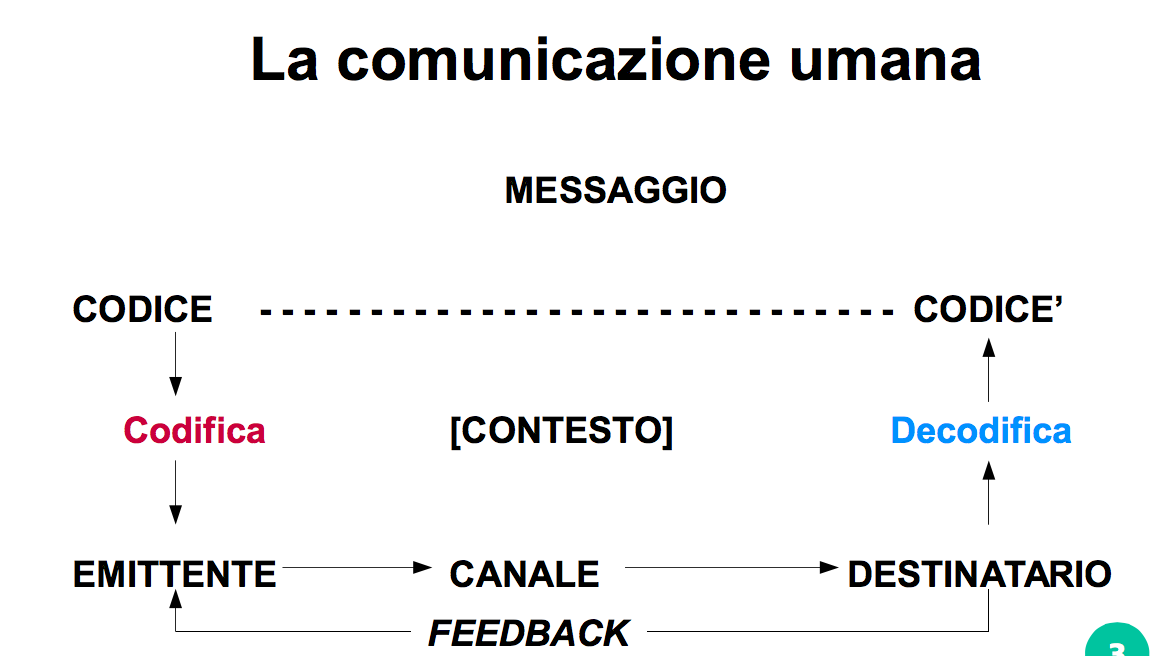
\includegraphics[width=.5\textwidth]{../imgs/comunicazioneUmana.png}

% L’applicazione di tecnologie informatiche nelle discipline umani- stiche, e in particolare nelle scienze letterarie, ha come suo fondamento la rappresentazione degli oggetti che costituiscono il loro dominio di studio. Tali oggetti sono in linea generale i testi.

% l’analisi del processo di scoperta e rappresentazione dell’oggetto testo e della sua struttura non può prescindere da una de- terminazione di cosa si intenda per testo, o quantomeno da una assun- zione implicita sulla sua natura;

% Il testo è un oggetto complesso in quanto è in grado di veicolare si- gnificato (e di rivestire dunque interesse scientifico) su più livelli strutturali, anche attraverso l’instaurazione di molteplici relazioni tra più livelli.

% Non possediamo nessuna teoria sufficientemente completa del testo

% Il fatto è che la rappresentazione (e a maggior ragione l’elaborazione) informatica è ontologicamente formale in senso stret- to.

% Il termine “testo”  si riferisce a un oggetto complesso e plurale, in cui esiste 
- un livello materiale, il supporto e le tracce d’inchiostro, 
- un livello astratto, la sequenza verbale, la quale a sua volta genera una serie di livelli di contenuti semantici.

% Lo studio del sapere ha come oggetto immediato i testi (letterari e non). Nella nostra cultura la quasi totalità dei testi letterari (fino a questo momento) è costituita da testi scritti su supporti cartacei di varia natura e forma.

% A questa struttura rigida del codice nell’ambito informatico (codice binario) va confrontata la complessa intersezione di codici che costituiscono un testo (da memorizzare).

% il termine “testo” non denota una entità acritica, oggetto della memorizzazione, affermando banalmente si tratta di una entità informativa complessa.

% Molteplici teorie del testo, quasi tutte sbilanciate sul livello verbale-semantico (linguistica testuale)

% Possiamo concludere che il testo è l’invariante, la successione di valori, rispetto alle variabili dei caratteri, della scrittura.
% Il testo è dunque una successione fissa di significati grafici (Segre, 1985).

% il testo come una entità astratta invariante, che in ogni operazione di realizzazione materiale della sequenza di simboli grafici determina la struttura fisica di un og- getto sensibilmente concreto (ovvero capace di attivare uno dei canali recettivi dell’uomo verso stimoli esterni), che costituisce il supporto materiale, stabile e riproducibile dell’informazione testuale. Distin- gueremo questo oggetto dal testo chiamandolo documento.

% Testo vs Documento

% oltre alla sequenza di grafemi, a un testo nel senso da noi indicato possono essere ascritte anche le segmentazioni logiche e le partizioni interne di interi blocchi
% il testo ha una certa struttura, i cui elementi sono determinati dalla struttura logico semantica del discorso,

% esiste anche un modello documento
% possibilità significative che derivano da una semantizzazione esplicita degli elementi non verbali di un testo scritto.
% ruolo della disposizione tipografica e topografica del segno grafico nella pagina bianca

% quale concezione o modello ontologico del testo è implicata nella rappresentazione informatica?

% natura del testo: il testo è, in un senso importante, una “ordered hierarchy of content objects (OHCO)”, una gerarchia ordinata di oggetti di contenuto [DeRose et al., 1990:3]. Gli oggetti di contenuto testuale a cui si fa riferimento in questa teoria sono sostanzialmente le strutture editoriali astratte di cui si com- pone un testo. Essi sono gerarchici poiché alcuni degli oggetti testuali con- tengono altri, e ordinati in quanto esiste una relazione lineare tra due oggetti posti sul medesimo livello gerarchico.

% il genere determina gli elementi che costituiscono il testo, quindi il tipo di documento. Reciprocamente un genere testuale è individuato dalla classe di oggetti di contenuto che contiene.
% Su questo impianto teorico si è basata, ad esempio, la prima fase del lavoro della Text Encoding Initiative.
% Sono però stati riscontrati una serie di problemi di rappresentazione che costituiscono dei veri e propri controesempi. Ci sono moltissimi casi in cui non esiste assolutamente accordo tra gli specialisti dei testi nell’asserire l’appartenenza di un dato testo a un tipo piuttosto che a un altro.  Questi diversi insiemi di elementi di contenuto non possono essere ricondotti a una struttura gerarchica unitaria.

% classi di elementi testuali che si sovrappongono rompendo i confini della struttura gerarchica di un documento: esempio: struttura metrica e quella morfosintattica di un testo poetico.. (Esempio clavius righe e sentence). Questi elementi si comportano come se appartenessero a diverse gerarchie di oggetti testuali che si sovrappongo.
% Prospettiva analitica:  “ogni prospettiva analitica su un testo determina una struttura gerarchica di oggetti di contenuto”.
% Un corollario operativo di questa tesi è che se due elementi a e b si sovrappongono, allora essi appartengono a due diverse prospettive analitiche.

% Ma è vero che a ogni coppia di elementi che si sovrappongono cor- rispondono due distinte prospettive teoriche? occorrenza di alcuni oggetti testuali che, pur appartenendo ragionevolmente a una medesima pro- spettiva analitica si sovrappongono.
Se due oggetti testuali evidenziati da una prospettiva teorica si sovrap- pongono, allora essi appartengono rispettivamente a due sottoprospet- tive diverse della prospettiva teorica principale. Questa ultima revisione della teoria gerarchica abbandona qualsiasi assunto di tipo essenzialista. In questa ottica il testo diventa un sistema a più livelli, che corrispondono a diversi punti di vista dell’osservatore.
% • il testo è un oggetto reale dotato di una sua struttura che corrisponde alla struttura del linguaggio di rappresentazione;
% • la struttura o meglio le strutture del testo sono strutture gerar- chiche: le sottoprospettive, comunque esse siano definite, dan- no luogo a gerarchie.

% Alcune teorie avanzano la necessità di abbandonare l’assunto ontologico che il testo sia un oggetto reale del mondo, dotato di una struttura intrinseca: Il testo è dunque una entità che viene costruita e non scoperta e a- nalizzata dalla attività scientifica. soluzione interessante e intellettualmente stimolante alle aporie determinate dal- la teoria gerarchica del testo, specialmente nella tematizzazione del ruolo dell’osservatore nei processi di rappresentazione.

% cos'è il testo (uso comune):
%a) un documento materiale composto da fogli di carta rilegati (o spillati o semplicemente raccolti insieme da un nastro di carta) che contengono tracce di inchiostro variamente disposte (oltre a eventuali tracce di altri materiali)
%b) un discorso linguistico fissato tramite la scrittura su un docu- mento materiale
%c) un’opera dell’ingegno che viene costituita da quel discorso

% cos'è un testo (uso più specialistico)
% d) lo stato linguistico di un singolo testimone materiale di un’opera
% e) lo stato linguistico di un medesimo testimone di un’opera che presenta diverse lezioni identificabili
% f) una versione edita di un’opera
% g) una sequenza coerente di enunciati in una lingua naturale
% Teso è l'invariante rispetto ai segni, è la succesione di valori invariabili. Il testo, dunque è ciò che permane, l’invariante, in ogni operazione di riproduzione materiale della sequenza di simboli grafici.
% Questa definizione di testo come un oggetto astratto allografico sembra fornire un criterio di individuazione di un testo in base al prin- cipio di identità per sostituzione

OHCO: alla do- manda che cosa è un testo veramente rispondiamo che un testo è un oggetto linguistico astratto organizzato secondo una struttura gerar- chica ordinata di oggetti di contenuto. (Asserzione poi rilevatasi fallace). Ma l’idea di una preminenza della struttura gerarchica nella testualità ha mantenuto un ruolo descrittivo ed esplicativo essenziale.